% Homotopy groups


%%%%(c)
%%%%(c)  This file is a portion of the source for the textbook
%%%%(c)
%%%%(c)    Abstract Algebra: Theory and Applications
%%%%(c)    Copyright 1997 by Thomas W. Judson
%%%%(c)
%%%%(c)  See the file COPYING.txt for copying conditions
%%%%(c)
%%%%(c)
\chap{Homomorphisms of Groups}{Homomorphism}


In this chapter we will introduce homomorphisms, which are a powerful tool in the study of the structure of abstract groups. Our brief treatment only gives the reader a taste of this important topic, and the reader wanting to go deeper is encouraged to look at other algebra texts.
\bigskip

Thanks to Tom Judson for material used in this chapter.
 
\section{Preliminary examples}
\label{sec:Homomorphism:Introduction}

  
In the previous chapter we talked about isomorphisms, which are bijections between two groups that also preserve
the group operation. We've seen that isomorphic groups are essentially the ``same'' group (thinking groupwise). 

For instance, we saw that the integers mod 4 and the $4^{th}$ roots of unity were isomorphic (${\mathbb Z_4} \cong \langle i \rangle$)  by the following bijection (isomorphism):

% $f: {\mathbb Z_4} \longrightarrow \langle i \rangle$  that takes 
\begin{align*}
    0 \rightarrow 1 ,~~     1 \rightarrow i,~~    2 \rightarrow -1,~~   3 \rightarrow -i.
\end{align*}

The group operation is preserved by this bijection:  for instance, $1  \oplus 2=3$ maps to 
$i \cdot -1 = -i$.
%, since indeed $3=-i$ according to $f$.  And this works for whatever two elements you pick in ${\mathbb Z_4}$:  the sum mod 4 is equivalent to complex multiplication of their corresponding elements in  $\langle i \rangle$.  Or
In general, for $a,b \in {\mathbb Z_4}$ we have
$$f(a \oplus b) = f(a) \cdot f(b).$$

 Now let us think about the groups \emph{ ${\mathbb Z_8}$} and $\langle i \rangle$.  Do they have the same relationship?  Are they isomorphic? 

Well, there is \emph{one} immediate problem that comes up:  $|{\mathbb Z_8}| \neq |\langle i \rangle|$.  And as we saw in the Isomorphism chapter, there's no way then to create a bijection from ${\mathbb Z_8}$ to $\langle i \rangle$:  specifically, there is just no way to create a one-to-one function from a domain of 8 elements to a codomain of 4 elements; the number of elements have to match.  But  let's look at their Cayley tables:

\begin{table}[H]
\caption{\label{groups_Z8_add_table2}Addition table for ${\mathbb Z}_8$}{\small
\begin{center}
\begin{tabular}{c|cccccccc}
$\oplus$ & 0 & 1 & 2 & 3 & 4 & 5 & 6 & 7 \\
\hline
0        & 0 & 1 & 2 & 3 & 4 & 5 & 6 & 7 \\
1       & 1 & 2 & 3 & 4 & 5 & 6 & 7 & 0 \\
2       & 2 & 3 & 4 & 5 & 6 & 7 & 0 & 1\\
3       & 3 & 4 & 5 & 6 & 7 & 0 & 1 & 2\\
4       & 4 & 5 & 6 & 7 & 0 & 1 & 2 & 3\\
5       & 5 & 6 & 7 & 0 & 1 & 2 & 3 & 4\\
6       & 6 & 7 & 0 & 1 & 2 & 3 & 4 & 5\\
7       & 7 & 0 & 1 & 2 & 3 & 4 & 5 & 6\\
\end{tabular}
\end{center}
}
\end{table}

\begin{table}[H]
\caption{Cayley table for $\langle i \rangle$}
\label{4_roots_table2}
{\small
\begin{center}
\begin{tabular}{c|cccccccc}
$\cdot$ & 1 &$i$ & -1 & $-i$  \\
\hline
1        & 1 &$i$ & -1 &$-i$  \\
$i$       &$i$ & -1 & $-i$ & 1  \\
-1       & -1 & $-i$ & 1 & $i$ \\
$-i$       & $-i$ & 1 & $i$ & -1 \\

\end{tabular}
\end{center}
}
\end{table}  

While we can't say that ${\mathbb Z_8}$ and $\langle i \rangle$ are isomorphic, there  are some similarities in the patterns of their Cayley tables.  
Notice for instance the pattern of 2's in the upper left portion of the ${\mathbb Z_8}$ table. This matches exactly with the pattern of -1's in the $\langle i \rangle$ table. In fact, we can see that in both tables the entries in each ``anti-diagonal'' are all the same. 
% The rows of ${\mathbb Z_8}$, like the rows of  $\langle i \rangle$ (and for that matter ${\mathbb Z_4}$ and  $R_4$), each start with their ''own" element and move up ''one by one" through the rest of the elements in the groups.  So you end up with staggered ribbons of the elements in the order given by the column headers in both Cayley tables.  
This similarity in structure suggests a similarity in the behavior of the group operations.  
So although we can't create a bijection, could we possibly create another function that preserves the group operations?   

\begin{example}{Z_8_i homomorph}
Let's try to create a function from ${\mathbb Z_8}$ to $\langle i \rangle$ which preserves group operations.  Since there are twice as many elements  in ${\mathbb Z_8}$ as in $\langle i \rangle$,  it seems natural that 2 elements from  ${\mathbb Z_8}$ should each go to one element in $\langle i \rangle$.  The question then is, Which two?  
%For instance what in ${\mathbb Z_8}$ will be a $1$?  What in ${\mathbb Z_8}$ will be an $i$?
 Because of the nature of modular addition, it makes some sense to pick elements of ${\mathbb Z_8}$ that are spaced evenly throughout ${\mathbb Z_8}$ if we want them to correspond to the same action in $\langle i \rangle$.  So let's look at the function  $g: {\mathbb Z}_8 \rightarrow \langle i \rangle$  that takes 
\begin{align*}
    0,4 \overset{g}{\longrightarrow} 1 ,~~     1,5 \overset{g}{\longrightarrow} i,~~    2,6 \overset{g}{\longrightarrow} -1,~~   3,7 \overset{g}{\longrightarrow} -i,  
\end{align*}
\noindent
as shown in Figure~\ref{fig:homomorph1}.

\begin{figure}[htb]
	   \center{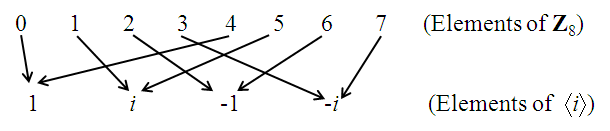
\includegraphics[width=4.in]
	         {images/homomorph1.png}}
	  \caption{\label{fig:homomorph1} Function $g$ between $\ZZ_8$ and $\langle i \rangle$. }
\end{figure}
\vspace{2 cm}

Let's take the  ${\mathbb Z_8}$ table then and start transforming it according to $g$.  First we replace all the elements of  ${\mathbb Z_8}$ with their counterparts in $\langle i \rangle$:

\begin{table}[H]
\caption{\label{groups_Z8_transfom1}First Transformation of ${\mathbb Z}_8$ into $\langle i \rangle$.}{\small
\begin{center}
\begin{tabular}{c|cccccccc}
$\oplus$ & 1 &$i$ & -1 & $-i$ & 1 & $i$ & -1 & $-i$ \\
\hline
1        & 1 & $i$ & -1 & $-i$ & 1 & $i$ & $-1$ & $-i$ \\
$i$       &$i$ & -1 & $-i$ & 1 & $i$ & -1 & $-i$ & 1 \\
-1       & -1 & $-i$ & 1 & $i$ & -1 & $-i$ & 1 & $i$\\
$-i$       & $-i$ & 1 & $i$ & -1 & $-i$ & 1 & $i$ & -1\\
1        & 1 & $i$ & -1 & $-i$ & 1 & $i$ & -1 & $-i$ \\
$i$       & $i$ & -1 & $-i$ & 1 & $i$ & -1 & $-i$ & 1 \\
-1       & -1 & $-i$ & 1 & $i$ & -1 & $-i$ & 1 & $i$\\
$-i$       & $-i$ & 1 & $i$ & -1 & $-i$ & 1 & $i$ & -1\\
\end{tabular}
\end{center}
}
\end{table}

Then we remove redundant rows/columns and change the group operation, and voil\`{a}:

\begin{table}[H]
\caption{\label{groups_Z8_transfom2}Second Transformation of ${\mathbb Z}_8$ into $\langle i \rangle$.}{\small
\begin{center}
\begin{tabular}{c|cccc}
$\cdot$ & 1 & $i$ & -1 & $-i$ \\
\hline
1        & 1 & $i$ & -1 & $-i$ \\
$i$       &$i$ & -1 & $-i$ & 1 \\
-1       & -1 & $-i$ & 1 & $i$ \\
$-i$       & $-i$ & 1 & $i$ & -1 \\

\end{tabular}
\end{center}
}
\end{table}

\noindent
This is exactly the Cayley table for  $\langle i \rangle$ (see Table~\ref{4_roots_table2}).  So $g$ does it! It preserves the group operations: if we take any two elements of ${\mathbb Z}_8$ and add them (say $3 \oplus 5 = 0$), the result is the same as taking their corresponding elements in $\langle i \rangle$ and multiplying them ($ -i \cdot i = 1$).  In other words, for all $a,b \in {\mathbb Z}_8$, 
\[
g(a \oplus b) = g(a) \cdot g(b).
\]
 
A bijection that preserved group operations was called an isomorphism.  So what do we call $g$?  We say that $g$ is a \emph{homomorphism} from ${\mathbb Z}_8$ to $\langle i \rangle$, and that ${\mathbb Z}_8$ is \emph{homomorphic} to $\langle i \rangle$.
\end{example}

We see some interesting things in  Example~\ref{example:Homomorphism:Z_8_i homomorph}. 
The elements in ${\mathbb Z}_8$ that map to 1 are  $0$ and $4$. The set $\{0,4\}$ is a subgroup of ${\mathbb Z}_8$.  Naturally it's a normal subgroup, since $\mathbb{Z}_8$ is abelian.
On the other hand, the sets $\{1,5\}, \{2,6\},$ and $\{3,7\}$ which map to $i, -1,$ and $-i$ respectively are \emph{not} subgroups of ${\mathbb Z}_8$. Instead, we may recognize them as the \emph{cosets} of $\{0,4\}$ in ${\mathbb Z}_8$. We saw in Section~\ref{subsec:Cosets:NormalSubAndFactorGroup:NormalSubgroups} 
that the cosets of a normal subgroup themselves form a group called the \emph{quotient group}. You may want
to go back and refresh your memory on the contents of that section before attempting the following exercise. 

%\begin{table}[H]
%\caption{Cayley table for ${\mathbb Z}_8/ \{0,4\}$}
%\label{Z8_04_factor}
%{\small
%\begin{center}
%\begin{tabular}{c|cccc}
%$\oplus$ & $\{0,4\}$ &$\{1,5\}$ &$\{2,6\}$ & $\{3,7\}$  \\
%\hline
%$\{0,4\}$   & $\{0,4\}$ &$\{1,5\}$ &$\{2,6\}$ & $\{3,7\}$  \\
%$\{1,5\}$  &$\{1,5\}$ &$\{2,6\}$ & $\{3,7\}$ & $\{0,4\}$  \\
%$\{2,6\}$   &$\{2,6\}$ & $\{3,7\}$  & $\{0,4\}$ &$\{1,5\}$ \\
%$\{3,7\}$  & $\{3,7\}$ & $\{0,4\}$ &$\{1,5\}$ &$\{2,6\}$  \\
%
%\end{tabular}
%\end{center}
%}
%\end{table}  

\begin{exercise}{verify_Z8/04}
Compute the Cayley table for ${\mathbb Z}_8/ \{0,4\}$. Label the rows and columns in the following order:
$\{0,4\}$,$\{1,5\}$, $\{2,6\}$,  $\{3,7\}$. 
\end{exercise}

This table possesses an eery similarity to another table that we've seen before:
%Notice that Table~\ref{Z8_04_factor} looks \emph{eerily} similar to the Cayley Table for $\langle i \rangle$, reprinted below: 
%
%\begin{table}[H]
%\caption{Cayley table for $\langle i \rangle$}
%\label{4_roots_table3}
%{\small
%\begin{center}
%\begin{tabular}{c|cccc}
%$\cdot$ & 1 &$i$ & -1 & $-i$  \\
%\hline
%1        & 1 &$i$ & -1 &$-i$  \\
%$i$       &$i$ & -1 & $-i$ & 1  \\
%-1       & -1 & $-i$ & 1 & $i$ \\
%$-i$       & $-i$ & 1 & $i$ & -1 \\
%
%\end{tabular}
%\end{center}
%}
%\end{table}  

\begin{exercise}{Z8/04_i_iso}
\begin{enumerate}[(a)]
\item
Compute the Cayley table for $\langle i \rangle$. Label the rows and columns in the following order:
$1$,$i$, $-1$,  $-i$. 
\item
By comparing Cayley tables, show that the function $h: {\mathbb Z}_8/\{0,4\} \longrightarrow \langle i \rangle$ is an isomorphism, where 
\begin{align*}
    \{0,4\} \overset{h}{\longrightarrow} 1 ,~~     \{1,5\}  \overset{h}\longrightarrow i,~~    \{2,6\}  \overset{h}\longrightarrow -1,~~   \{3,7\}  \overset{h}\longrightarrow -i.  
\end{align*}
\end{enumerate}
\end{exercise}

So ${\mathbb Z}_8/ \{0,4\} \cong \langle i \rangle$! (See Figure~\ref{fig:homomorph2}.) 

\begin{figure}[htb]
	   \center{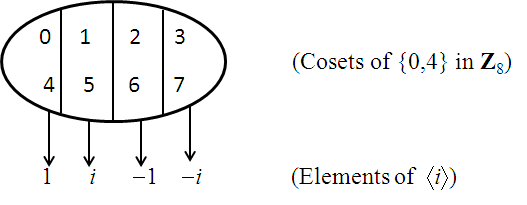
\includegraphics[width=3.in]
	         {images/homomorph2.png}}
	  \caption{\label{fig:homomorph2} Isomorphism $h$ between $\ZZ_8/\{0,4\}$ and $\langle i \rangle$. }
\end{figure}

Example~\ref{example:Homomorphism:Z_8_i homomorph} exhibited lots of interesting properties. Let's see if these properties hold for other examples as well. We may  then formalize our observations and provide proofs.

\begin{example}{Z_8_isub_homomorph}
The function $g$ which we constructed in Example~\ref{example:Homomorphism:Z_8_i homomorph} was not one-to-one, but it was onto. Is ``onto'' necessary? Or could we possibly find a function from ${\mathbb Z}_8$ to $\langle i \rangle$ that still preserves the group operation, whose range is not all of $\langle i \rangle$?  

%Essentially, we are asking ourselves the following: can we map the elements of ${\mathbb Z}_8$ to some, but not all, of the elements of $\langle i \rangle$ (a proper subset) in such a way that after we replace the elements in the ${\mathbb Z}_8$ table according to the function and remove all redundant rows and columns, we end up with some subset of the Cayley table for $\langle i \rangle$? 

Let's consider the function $q: {\mathbb Z}_8 \longrightarrow \langle i \rangle$  defined by: 
\begin{align*}
    0,2,4,6\overset{q}{\longrightarrow} 1 ,~~     1,3,5,7 \overset{q}{\longrightarrow} -1.
\end{align*}

\begin{exercise}{1,-1_subgroup}
Prove that $\{1,-1\}$ is a subgroup of $\langle i \rangle$.
\end{exercise}

If we relabel the Cayley table for ${\mathbb Z}_8$ according to $1$, we get the following:

\begin{table}[H]
\caption{\label{1,-1_Z8_transfom1}First Transformation of ${\mathbb Z}_8$ into $\{1,-1\}$.}{\small
\begin{center}
\begin{tabular}{c|cccccccc}
$\cdot$ & 1 &-1 & 1 & -1 & 1 & -1 & 1 & -1 \\
\hline
1         & 1 &-1 & 1 & -1 & 1 & -1 & 1 & -1 \\
-1      &-1 & 1 & -1 & 1 & -1 & 1 & -1 & 1  \\
1       & 1 &-1 & 1 & -1 & 1 & -1 & 1 & -1 \\
-1       &-1 & 1 & -1 & 1 & -1 & 1 & -1 & 1  \\
1        & 1 &-1 & 1 & -1 & 1 & -1 & 1 & -1 \\
-1        &-1 & 1 & -1 & 1 & -1 & 1 & -1 & 1  \\
1      & 1 &-1 & 1 & -1 & 1 & -1 & 1 & -1 \\
-1      &-1 & 1 & -1 & 1 & -1 & 1 & -1 & 1  \\
\end{tabular}
\end{center}
}
\end{table}

And then if we remove the redundant rows and columns, we get:

\begin{table}[H]
\caption{\label{1,-1_Z8_transfom2}Second Transformation of ${\mathbb Z}_8$ into $\{1,-1\}$.}{\small
\begin{center}
\begin{tabular}{c|cc}
$\cdot$ & 1 & -1  \\
\hline
1        & 1 & -1  \\
-1       & -1 & 1 \\
\end{tabular}
\end{center}
}
\end{table}

Now this isn't the \emph{whole} Cayley table for $\langle i \rangle$ (Table~\ref{groups_Z8_transfom2}), but it \emph{is} the part of the Cayley table that corresponds to the elements 1 and -1 (remove rows 2 and 4 as well as columns 2 and 4).  So $q$  preserves the operations between $\ZZ_8$ and $\langle i \rangle$, since for all $a,b \in {\mathbb Z}_8$ we have
\[
q(a \oplus b) = q(a) \cdot q(b).
\]
In other words, $q$ is a homomorphism.
\end{example}

In Example ~\ref{example:Homomorphism:Z_8_isub_homomorph} we find several similarities to \ref{example:Homomorphism:Z_8_i homomorph}:

\begin{itemize}
\item
The set $\{0,2,4,6\} \subset {\mathbb Z}_8$ which maps to  the identity of $\langle i \rangle$ is a  normal subgroup of  ${\mathbb Z}_8$. (We will use $H$ to denote this subgroup.)
\item
The set $\{1,3,5,7\}$ which maps to $-1$  is a coset of $H$ in ${\mathbb Z}_8$. (We may write $\{1,3,5,7\}$ as $1+H$).

\item
We may use the homomorphism $q$ to construct an isomorphism, as you will show in the following exercise.

\begin{exercise}{Z8/0246_1-1_iso}
\begin{enumerate}[(a)]
\item
Create the Cayley Table for the quotient group ${\mathbb Z}_8/ H$.
\item
Show that the function from ${\mathbb Z}_8/ H$  to $\langle i \rangle$  which maps
\begin{align*}
   H \longrightarrow 1 ,~~     1+H \longrightarrow -1
\end{align*}
is an isomorphism from ${\mathbb Z}_8/ H$ to the subgroup $\{1,-1\}$ of $ \langle i \rangle$.
\end{enumerate}
\end{exercise}

\end{itemize}


\section{Definition and several more examples}
\label{sec:Homomorphism:Definitions}

In  the previous section we saw that homomorphisms give us a way of finding structural similarity between groups, even when those groups are not isomorphic.  A homomorphism only needs to  map elements from one group to another in such a way that it preserves the operations between the two groups.  That's it. Unlike isomorphisms, it doesn't have to be one-to-one or onto.  

Let's now formally state the definition:

\begin{defn}{homomorphism_def}
A
\term{homomorphism}\index{Group!homomorphism of}\index{Homomorphism} between groups $(G, \cdot)$ and $(H, \circ)$ is a function $f :
G \rightarrow H$ such that  
\[
f( g_1 \cdot g_2 ) = f( g_1 ) \circ f( g_2 )
\]
for all $g_1, g_2 \in G$. The range of $f$ in $H$ is called the \term{
homomorphic image}\index{Homomorphic image}~of~$f$.
\footnote{You may have noticed that in the Isomorphisms chapter we used Greek letters ($\phi$ etc.) for isomorphisms, whereas here we typically use the  letter $f$ to denote a homomorphism. There is no special reason for this--both notations are used in math books, and you should be comfortable either way.}
 \end{defn}

\begin{exercise}{homo_image_kernel_1}

\begin{enumerate}[(a)]
\item
For the homomorphism $g$ from ${\mathbb Z}_8$ to $\langle i \rangle$ in Example~\ref{example:Homomorphism:Z_8_i homomorph}, what is the homomorphic image of $g$?
\item
For the homomorphism $q$ from ${\mathbb Z}_8$ to $\langle i \rangle$ in Example~\ref{example:Homomorphism:Z_8_isub_homomorph}, what is the homomorphic image of $q$?
\end{enumerate}
\end{exercise}  
 
%Homomorphisms can be used to bring out relationships between groups that are not exactly identical, but nonetheless are structurally similar in some way.  For example, the symmetric group $S_n$ and the group ${\mathbb
%Z}_2$ are related by the fact that $S_n$ can be divided into even and
%odd permutations that exhibit a group structure like that ${\mathbb
%Z}_2$, as shown in the following multiplication table. 
%\begin{center}
%\begin{tabular}{c|cc}
    %        & even & odd \\
%\hline
%even & even & odd \\
%odd  & odd  & even
%\end{tabular}
%\end{center}
%We use homomorphisms to study relationships such as the one we have
%just described.
 
 All of our examples so far have been with finite groups; let's look at infinite groups instead.  As we saw in the Isomorphisms chapter, with finite groups we can use Cayley tables to verify the equality of the group operations, but with infinite groups we don't have  Cayley tables, so we need to use  the definition of a homomorphism.

\begin{example}{homo_T}
Recall that the circle group ${ \mathbb T}$ consists of all complex numbers $z$ such that $|z|=1$. So geometrically, the circle group consists of the complex numbers that trace out a circle of radius 1 about the origin in the complex plane (hence the name), as shown in the figure below:

\begin{figure}[hbt]
\begin{center}
\tikzpreface{cyclic_roots_unity}
\begin{tikzpicture}[scale=1.65] %Replaced figure with tikz figure - TWJ 5/6/2010

\draw [->]  (0,-1.5) -- (0,1.5);
\draw  [->] (-1.75,0) -- (1.75,0);
\node [right] at (0,1.5) {Im};
\node [below] at (1.75,0) {Re};
\node [below] at (0.1,0) {$0$};

\draw (0,0) circle (1);

\filldraw[fill=black, draw=black] (0:1) circle (0.03);
\filldraw[fill=black, draw=black] (90:1) circle (0.03);
\filldraw[fill=black, draw=black] (180:1) circle (0.03);
\filldraw[fill=black, draw=black] (270:1) circle (0.03);


\node [right] at (1,-0.15) {1};
\node [left] at (0,1.15) {$i$};
\node [left] at (-1,-0.15) {$-1$};
\node [left] at (0,-1.15) {$-i$};

\end{tikzpicture}

\end{center}
\caption{Circle group ${ \mathbb T}$ in complex plane}
\label{fig:circleGroup}
\end{figure}

\noindent
Now imagine wrapping the real number line around this circle like it was a tape measure, with $0$ on the real number line corresponding to $1$ on the unit circle.  Then we would have a correspondence between each real number and a complex number in ${ \mathbb T}$. Every $2\pi$ units the real numbers start around the circle again, so that an infinite set of real numbers corresponds to each complex number $z$ in ${ \mathbb T}$.  For instance not only 0, but $2\pi, 4\pi, 6\pi$, etc. would correspond to $1$.  
Evidently for a given complex number $z$, any real number $\alpha$ that corresponds to $z$ is an \emph{argument} for $z$ (see Figure~\ref{fig:polarcoord}), so that $z = \cis \alpha$.
From this point of view, we may conceive of $\cis$ as  a function from ${ \mathbb R}$ to  ${ \mathbb T}$.   Does $\cis$ preserve the operations between ${ \mathbb R}$ and ${ \mathbb T}$? We've shown this before in Proposition~\ref{proposition:ComplexNumbers:polar_mult} in the Complex Numbers chapter, but it won't hurt to see it again:
\begin{align*}
\cis( \alpha + \beta )
& =
\cos( \alpha + \beta ) + i \sin( \alpha + \beta ) \\
& =
(\cos \alpha \cos \beta - \sin \alpha \sin \beta)  + i( \sin \alpha 
\cos \beta + \cos \alpha \sin \beta ) \\
& =
(\cos \alpha + i \sin \alpha )(\cos \beta + i \sin \beta
) \\
& = \cis( \alpha ) \cis( \beta ).
\end{align*}
So we have it; $\cis$ is a homomorphism from the additive group of real numbers to the circle group.
This means that in some sense, complex multiplication on the unit circle is like addition of real numbers.
\end{example}


In the following exercise, we relate the previous example to the properties observed in  Examples~\ref{example:Homomorphism:Z_8_i homomorph} and~\ref{example:Homomorphism:Z_8_isub_homomorph} in the previous section.

\begin{exercise}{circle_cosets_factorgroup}
As we mentioned above, $\cis$ maps $0, \pm 2\pi, \pm 4\pi$, etc to $1$, the identity, in ${ \mathbb T}$. Another way to say the same thing is:

$\cis^{-1}(1) = \{ \ldots , -4\pi, -2\pi, 0, 2\pi, 4\pi, \ldots \}$.

\begin{enumerate}[(a)]
\item
Prove that $\{ \ldots , -4\pi, -2\pi, 0, 2\pi, 4\pi, \ldots \}$ is a normal subgroup of ${ \mathbb R}$
\item
What are the cosets of $\{ \ldots , -4\pi, -2\pi, 0, 2\pi, 4\pi, \ldots \}$ in ${ \mathbb R}$?
\item
Define a function $F:{ \mathbb R} / 2\pi { \mathbb Z} \rightarrow { \mathbb T}$ by:  $F(x + 2\pi\mathbb{Z}) = \cis(x)$. Show that the function is well-defined:  that is, show that if  $x_1$ and $x_2$ are both elements of the same coset of $2\pi\mathbb{Z}$, then $F(x_1+2\pi\mathbb{Z}) = F(x_2+2\pi\mathbb{Z})$.
\item
Show that $F$ defined above is a bijection: that is, $F$ maps different cosets to different elements of $\mathbb{T}$.
\item
Show that $F$ defined above is an isomorphism.
\item
What is the homomorphic image of the function $\cis: \mathbb{R} \rightarrow \mathbb{T}$?
\end{enumerate}
\end{exercise} 

\begin{example}{homo_C*}
The circle group ${ \mathbb T}$ also gives us a completely different way of constructing a homomorphism between complex and real numbers.  Every complex number in ${ \mathbb T}$ has modulus 1; i.e. they lie all on a circle of radius 1 in the complex plane.  If we increase radius of the circle to 2, all of those complex numbers have the same modulus 2.  In fact if you keep increasing or decreasing the radius of the circle, you can catch all the complex numbers in the plane with the concentric circles you've created.  So every complex number (except 0) corresponds to a positive real number by its modulus. Since we can represent any complex number as $r \cis \theta$, we can define a function
$f:  {\mathbb C}^\ast \mapsto  {\mathbb R}^\ast$ by

\[
f(r \cis \theta) = r.
\]
Let's see whether $f$ is a homomorphism. If $r_1 \cis \theta_1$ and $r_2 \cis \theta_2$ are arbitrary nonzero complex numbers, we have:
\begin{align*}
f((r_1\cis \theta_1)\cdot (r_2\cis \theta_2)) &= f(r_1 \cis \theta_1 r_2 \cis \theta_2)\\
&= f((r_1 r_2)\cis (\theta_1+ \theta_2))\\
&= r_1 r_2 \\
&= f((r_1\cis \theta_1)\cdot f(r_2\cis \theta_2)).
\end{align*}
So $f$ is indeed a homomorphism from ${\mathbb C}^\ast$ to ${\mathbb R}^\ast$.
\end{example}
Once again, we may compare this example to the remarks of the previous section.

\begin{exercise}{Cstar_modulus_cosets}
With reference to the function $f$ defined in Example~\ref{example:Homomorphism:homo_C*}:
\begin{enumerate}[(a)]
\item
What is the homomorphic image of $f$?
\item
Prove that the homomorphic image of $f$ is a subgroup of ${\mathbb R}^\ast$.
\item
Find all the elements in ${\mathbb C}^\ast$ that map  to the identity in ${\mathbb R}^\ast$; that is, find all $r \cis \theta \in {\mathbb C}^\ast$ such that $f(r \cis \theta) = 1$.
\item
Is the set from part (b) a normal subgroup of ${\mathbb C}^\ast$?  Prove or disprove.
\item
What are the cosets in ${\mathbb C}^\ast$ of the set in part (b)?
\item
Define the quotient group created by the normal subgroup in (e), and prove that it's isomorphic to  the homomorphic image of $f$.
\end{enumerate}
\end{exercise}
 

Now it's your turn. In the following exercises, you'll have a chance  to verify some homomorphisms for yourself.

\begin{exercise}{homo_GL2}
Consider the group $GL_2( {\mathbb R })$ (that is, the group of invertible $2 \times 2$ matrices under matrix multiplication). If
\[
A=
\begin{pmatrix}
a & b \\
c & d
\end{pmatrix}
\]
is in $GL_2( {\mathbb R })$, then the determinant is  nonzero; that is, $\det(A) = ad -bc
\neq 0$.  

\begin{enumerate}[(a)]
\item
Prove that $\det( AB) = \det(A) \det(B)$ for $A, B \in GL_2( {\mathbb R}
)$. This shows that the function $\det$ is a homomorphism from $ GL_2( {\mathbb R })$ to ${\mathbb R}^\ast$.

\item
What is the homomorphic image of $\det$?
\item
In the Groups chapter we defined $SL_2( {\mathbb R })$ as the set of $2 \times 2$ real matrices whose determinant is 1. It follows that $SL_2( {\mathbb R })$ is the subset of $GL_2( {\mathbb R })$ which maps under $\det$ to the identity of $\RR^*$. Prove that $SL_2( {\mathbb R })$ is a subgroup of $GL_2( {\mathbb R })$.
\item
Describe the cosets of $SL_2( {\mathbb R })$ in $GL_2( {\mathbb R })$.
\item
Prove that $SL_2( {\mathbb R })$ is a normal subgroup of $GL_2( {\mathbb R })$. 
\hyperref[sec:Homomorphism:Hints]{(*Hint*)} 
\item
Prove that the quotient group $GL_2( {\mathbb R }) / SL_2( {\mathbb R })$ is isomorphic to ${\mathbb R}^\ast$.
\end{enumerate}  
\end{exercise}

\begin{rem}
This last exercise wasn't as easy to visualize as the previous ones.  So we had to rely on \emph{properties} rather than intuition. This is typically what happens in mathematics: you start with visualizable examples, and use these as a springboard to leap into higher abstractions.
\end{rem}

\begin{exercise}{homo_GL2_a}
\begin{enumerate}[(a)]
\item
Define a function $f: {\mathbb C} \rightarrow {\mathbb R }$ as follows: $f(a+bi) = a$.  Prove or disprove:  $f$ is a  homomorphism.
\item
Define a function $g: {\mathbb C} \rightarrow {\mathbb R }$ as follows: $g(a+bi) = b$.  Prove or disprove:  $g$ is a homomorphism.
\item
Define a function $h: {\mathbb C}^* \rightarrow {\mathbb R }^*$ as follows: $h(a+bi) = a$.  Prove or disprove:  $h$ is a  homomorphism. (\emph{Note} this is a different situation from part (a)!) 
\end{enumerate}
\end{exercise}

\begin{exercise}{2x2_add}
Remember that  ${\mathbb M}_2( {\mathbb R})$ is the group of real-valued $2 \times 2$ matrices under addition.  Define and prove a homomorphism from ${\mathbb M}_2( {\mathbb R})$ to ${\mathbb R}$.
\end{exercise}

Now lets deal with homomorphisms in a more general context, to prepare us for the task of proving  properties of homomorphisms in general (which we'll get to in the next section).
 
\begin{exercise}{homo_Zn}
Let $G$ be a group and $g \in G$. In the Groups chapter we saw that the set of all integer powers (positive, negative, and zero) of $g$ form a group, which is called the
\emph{cyclic subgroup} generated by $g$ and is denoted by $\langle g \rangle$. 
Since each integer corresponds to a power of $g$, we may define a map $f : {\mathbb Z}
\rightarrow G$ by $f( n ) = g^n$. 
\begin{enumerate}[(a)]
\item
Show that $f$ is a group
homomorphism.
\item 
What is the homomorphic image of $f$?
\item
Find all the elements in ${\mathbb Z}$ that map  to the identity in $G$.
\item
Is the set from part (c) a subgroup of ${\mathbb Z}$?  Prove or disprove.
\item
What are the cosets in ${\mathbb Z}$ of the set in part (c)?
\item
Show the set in part (c) is a normal subgroup in ${\mathbb Z}$.
\item
Define the quotient group created by the normal subgroup in (g), and prove that it's isomorphic to  the homomorphic image of $f$.
\end{enumerate}
\end{exercise}


 
\begin{exercise}{}
If $G$ is an abelian group and $n \in {\mathbb N}$, show that $\phi : G
\rightarrow G$  defined by $\phi(g) = g^n$ is a group homomorphism.  
\end{exercise}

Finally, let's look at one more pattern for the homomorphisms we've developed so far before we go proving these patterns/properties hold for homomorphisms of groups in general:

\begin{exercise}{homo_ex_inverses}
\begin{enumerate}[(a)]
\item
In the group ${\mathbb Z}_8$, the inverse of 3 is 5 (we may write this as $3^{-1} = 5$).  Using the homomorphism $g$ from Example~\ref{example:Homomorphism:Z_8_i homomorph}, what is $g(5)$?  What is the inverse of $g(3)$ in the group $\langle i \rangle$? What does this example show about the relation between $g(3^{-1})$ and $(g(3))^{-1}$?
\item
In ${\mathbb Z}_8$, $2^{-1} = 6$.  Using the homomorphism $q$ from Example~\ref{example:Homomorphism:Z_8_isub_homomorph}, what is $q(2^{-1})$?  What is $(q(2))^{-1}$? What do you notice about your two answers?
\item
In  ${\mathbb C}^\ast$, $(r \cis \theta)^{-1} = \frac{1}{r} \cis (2\pi - \theta)$.  Using $f$ from Example~\ref{example:Homomorphism:homo_C*},  compute $f\left((r \cis \theta)^{-1}\right)$ and $(f(r \cis \theta))^{-1}$. What do you notice about your two answers? 
\item
In $GL_2( {\mathbb R })$, what is the inverse of
$\begin{pmatrix}
a & b \\
c & d
\end{pmatrix}$?
Using $f$ from Exercise~\ref{exercise:Homomorphism:homo_GL2}, does $f\left((\begin{pmatrix} a & b \\ c & d \end{pmatrix})^{-1}\right) = [f(\begin{pmatrix} a & b \\ c & d \end{pmatrix})]^{-1}$?  Verify or give a counterexample.
\item
What general property of homomorphisms can you infer from these examples? (You don't need to give a proof if you don't want to.)
\end{enumerate}
\end{exercise}


%\begin{exercise}
%Show that a homomorphism defined on a cyclic group is completely
%determined by its action on the generator of the group.
%\end{exercise}




 

%\begin{exercise}
%Let $A$ be an $m \times n$ matrix.  Show that matrix multiplication,
%$x \mapsto Ax$, defines a homomorphism $\phi : {\mathbb R}^n \rightarrow
%{\mathbb R}^m$. 
%\end{exercise}
 

\section{Proofs of homomorphism properties}
\label{sec:Homomorphism:ProofProperties}

So it seems there are several properties of homomorphisms that have consistently held true in our examples so far.  
For any  homomorphism $f$ with domain $G$ and the codomain $H$, it seems that:


\begin{itemize}
\item
The elements in $G$ that map under $f$ to the identity of $H$ are in fact a normal subgroup of $G$.
\item
The quotient group created by that normal subgroup is then isomorphic to the image of the homomorphism.
\item
If $f$ maps $g$ to $h$, then $f$ also maps $g^{-1}$ to $h^{-1}$.
\end{itemize}

These properties are indeed true for all homomorphisms, and we'll take the next two sections to prove these as well as other properties of homomorphisms.  
We begin with 
 
\begin{prop}{HomorphismSubgroupProp}
Let $f : G \rightarrow H$ be a homomorphism of groups. Then 
\begin{enumerate}
 
\item
If $e$ is the identity of $G$, then $f( e)$ is the identity of
$H$;  
 
\item
For any element $g \in G$, $f( g^{-1}) = [f( g )]^{- 1}$;
 
\item
If $S$ is a subgroup of $G$, then $f(S )$ is a subgroup of
$H$;
 
\item \label{normal_kernel}
If $T$ is a  subgroup of $H$, then $f^{-1}(T) = \{ g \in G :
f(g) \in T \}$ is a subgroup of $G$. Furthermore, if $T$ is
normal in $H$, then $f^{-1}(T)$ is normal in $G$. 
 
\end{enumerate}
\end{prop}
 
 
\begin{proof}

%Since we're proving these properties for groups in general, we can't take advanatage of specific properties of say complex numbers, matrices, real numbers, etc. like we have been so far.  Instead,we must rely on the properties of groups in general. Let's start.
 
(1)
Suppose that $e$ and $e'$ are the identities of $G$ and $H$,
respectively. Then
\[
e' f(e) = f(e) = f(e e) = f(e) f(e).
\]
By cancellation, $f(e) = e'$.
 
 
(2)
This statement follows from the fact that
\[
f( g^{-1}) f(g) = f(g^{-1} g) = f(e) = e.
\]
 
 
(3)
The set $f(S)$ is nonempty since the identity of $T$ is in
$f(S)$.
Suppose that $S$ is a subgroup of $G$ and let $x$ and $y$ be in
$f(S)$. There exist elements $a, b \in S$ such that $f(a) =
x$ and $f(b)=y$. Since 
\[
xy = f(a) f(b) = f(a b ) \in f(S),
\]
and
\[
x^{-1} = f(a)^{-1} = f(a^{-1}) \in f(S),
\]
it follows that $f(S)$ is a subgroup of $H$ (since it is closed under the group operation and inverse).
  
(4)
Let $T$ be a subgroup of $H$ and define $S$ to be
$f^{-1}(T)$; that is, $S$ is the set of all $g \in G$ such
that $f(g) \in T$.  The identity is in $S$ since $f(e) = e$.
If $a$ and $b$ are in $S$, then $f(ab^{-1}) = f(a)[ f(b)
]^{-1}$ is in $T$ since $T$ is a subgroup of $H$.  Therefore,
$ab^{-1} \in S$ and $S$ is a subgroup of $G$. If $T$ is normal
in $H$, we must show that $g^{-1} h g \in S$ for $h \in S$ and
$g \in G_1$. But 
\[
f( g^{-1} h g) = [ f(g) ]^{-1} f( h ) f( g ) \in
T,
\]
since $T$ is a normal subgroup of $H$.  Therefore, $g^{-1}hg \in
S$.\index{Normal subgroup}
\end{proof}

Now that we have these properties down, we can use them to prove some other properties of homomorphisms.  
We know that homomorphisms preserve  group operations, which suggests that homomorphisms may preserve other group properties as well. We'll look at two group properties in the next exercise.

 
\begin{exercise}{homo_abelian_cyclic}
Prove the following:
\begin{enumerate}[(a)]
\item
If $f : G \rightarrow H$ is a group homomorphism and $G$ is
abelian, prove that $f(G)$ is also abelian. 
 
\item
If $f : G \rightarrow H$ is a group homomorphism and $G$ is cyclic,
prove that $f(G)$ is also cyclic. 
\end{enumerate}
\end{exercise} 

\medskip

One of the patterns we saw in our examples that we haven't verified yet was that the elements in $G$ that map to the identity of $H$ formed a normal subgroup in $G$.  We can now prove this in general, but first a definition:
 
\begin{defn}{defkernel} 
Let $f : G \rightarrow H$ be a  homomorphism and suppose that
$e_H$ is the identity of $H$. 
The set  $f^{-1} ( \{ e_H \})$ is  called the \term{
kernel}\index{Kernel!of a
homomorphism}\index{Homomorphism!kernel} of $f$, and will
be denoted by $\ker f$\label{kernelofphi}. 
\end{defn}
 
 
\begin{prop}{homo_ker_normal}
Let $f : G \rightarrow H$ be a group homomorphism. Then the kernel
of $f$ is a normal subgroup of $G$.\index{Kernel!as a normal subgroup} 
\end{prop}

\begin{exercise}{hker}
Prove Proposition~\ref{proposition:Homomorphism:homo_ker_normal}. 
\hyperref[sec:Homomorphism:Hints]{(*Hint*)} 
\end{exercise}

\begin{exercise}{ker_review}
What were the kernels of the homomorphisms in:
\begin{enumerate}[(a)]
\item
Example~\ref{example:Homomorphism:Z_8_i homomorph}
\item
Example~\ref{example:Homomorphism:Z_8_isub_homomorph}
\item
Example~\ref{example:Homomorphism:homo_T}
\item
Example~\ref{example:Homomorphism:homo_C*}
\item
Exercise~\ref{exercise:Homomorphism:homo_GL2}
\end{enumerate}
\end{exercise} 
 
%\begin{example}{homo_G2_to_R}
%Let us examine the homomorphism $\phi : GL_2( {\mathbb R }) \rightarrow
%{\mathbb R}^\ast$ defined by $A \mapsto \det( A )$. Since 1 is the
%identity of ${\mathbb R}^\ast$, the kernel of this homomorphism is all
%$2 \times 2$ matrices having determinant one. That is, $\ker \phi =
%SL_2( {\mathbb R })$.
%\mbox{\hspace{1in}}
%\end{example}
 
 
%\begin{example}{kernel}
%The kernel of the group homomorphism $\phi : {\mathbb R} \rightarrow
%{\mathbb C}^\ast$ defined by $\phi( \theta ) = \cos \theta + i \sin
%\theta$ is $\{ 2 \pi n : n \in {\mathbb Z} \}$. Notice that $\ker \phi
%\cong {\mathbb Z}$. 
%\end{example}
 
%\begin{example}{homo_g^n}
%Let $G$ be a group. Suppose that  $g \in G$ and $\phi$ is the
%homomorphism from ${\mathbb Z}$ to $G$ given by $\phi( n ) = g^n$. If the
%order of $g$ is infinite, then the kernel of this homomorphism is $\{
%0 \}$ since $\phi$ maps ${\mathbb Z}$ onto the cyclic subgroup of $G$
%generated by $g$. However, if the order of $g$ is finite, say $n$,
%then the kernel of $\phi$ is $n {\mathbb Z}$.
%\end{example}

 
 %\begin{example}{homo_g^n}
%Let $G$ be a group. Suppose that  $g \in G$ and $\phi$ is the
%homomorphism from ${\mathbb Z}$ to $G$ given by $\phi( n ) = g^n$. If the
%order of $g$ is infinite, then the kernel of this homomorphism is $\{
%0 \}$ since $\phi$ maps ${\mathbb Z}$ onto the cyclic subgroup of $G$
%generated by $g$. However, if the order of $g$ is finite, say $n$,
%then the kernel of $\phi$ is $n {\mathbb Z}$.
%\end{example}
 

\begin{exercise}{}
Which of the following functions are homomorphisms? If the map is a
homomorphism, what is the kernel? 
\begin{enumerate}
 
%\item
%$\phi : {\mathbb R}^\ast \rightarrow GL_2 ( {\mathbb R})$ defined by
%\[
%\phi( a ) =
%\left(
%\begin{array}{cc}
%1 & 0 \\
%0 & a
%\end{array}
%\right)
%\]
 
\item
$f : {\mathbb R} \rightarrow GL_2 ( {\mathbb R})$ defined by
\[
f( a ) =
\left(
\begin{array}{cc}
1 & 0 \\
a & 1
\end{array}
\right)
\]
 
\item
$f : GL_2 ({\mathbb R})   \rightarrow {\mathbb R}$ defined by
\[
f
\left(
\left(
\begin{array}{cc}
a & b \\
c & d
\end{array}
\right)
\right)
= a + d
\]
 
%\item
%$\phi : GL_2 ( {\mathbb R})   \rightarrow {\mathbb R}^\ast$ defined by 
%\[
%\phi
%\left(
%\left(
%\begin{array}{cc}
%a & b \\
%c & d
%\end{array}
%\right)
%\right)
%= ad -bc
%\]
 
\item
$f : {\mathbb M}_2( {\mathbb R})   \rightarrow {\mathbb R}$ defined by
\[
f
\left(
\left(
\begin{array}{cc}
a & b \\
c & d
\end{array}
\right)
\right)
= b,
\]
where ${\mathbb M}_2( {\mathbb R})$ is the additive group of $2 \times
2$ matrices with entries in ${\mathbb R}$.
 
\end{enumerate}
\end{exercise}

\begin{exercise}{}
Let $f : {\mathbb Z} \rightarrow {\mathbb Z}$ be given by $f(n) = 7n$.
Prove that $f$ is a group homomorphism. Find the kernel and the
image of $f$.
\end{exercise} 
 
\begin{example}{homo_Z7}
Suppose that we wish to determine all possible homomorphisms $f$
from ${\mathbb Z}_7$ to  ${\mathbb Z}_{12}$. Since the kernel of $f$ must
be a subgroup of  ${\mathbb Z}_7$, there are only two possible
kernels, $\{ 0 \}$ and all of ${\mathbb Z}_7$.  The image of a subgroup
of ${\mathbb Z}_7$ must be a subgroup of ${\mathbb Z}_{12}$. Hence, there is
no injective homomorphism; otherwise, ${\mathbb Z}_{12}$ would have a
subgroup of order 7, which is impossible. Consequently, the only
possible homomorphism from ${\mathbb Z}_7$ to  ${\mathbb Z}_{12}$ is the one
mapping all elements to zero. 
\end{example}

\begin{exercise}{}
Describe all of the homomorphisms from ${\mathbb Z}_{24}$ to ${\mathbb
Z}_{18}$. 
\end{exercise} 
 
\begin{exercise}{}
Describe all of the homomorphisms from ${\mathbb Z}$ to ${\mathbb Z}_{12}$. 
\end{exercise} 

\begin{exercise}{allhom}
Find all of the homomorphisms $f : {\mathbb Z} \rightarrow {\mathbb Z}$.
Which of these are isomorphisms?
\hyperref[sec:Homomorphism:Hints]{(*Hint*)} 
\end{exercise} 

 
\section{The First Isomorphism Theorem}
\label{sec:Homomorphism:FirstIsomorphismTheorem}
 
There's one property that we observed in earlier sections of this chapter that we haven't proven so far, namely,  the quotient group created by the kernel of a homomorphism is isomorphic to the image of the homomorphism.  In order to do this, we'll need a clearer idea of how homomorphisms actually work. Figure~\ref{fig:homomorph3} gives a schematic diagram of a general homomorphism $f$ with kernel $K$. 
\begin{figure}[htb]
	   \center{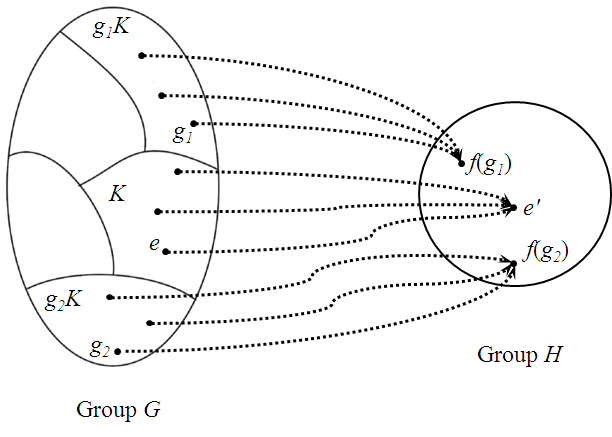
\includegraphics[width=4.in]
	         {images/homomorph3.png}}
	  \caption{\label{fig:homomorph3} Homomorphism $f:G \rightarrow H$ with kernel $K$. }
\end{figure}


The figure shows the cosets of $K$, which form a partition of $G$ as we showed in the Cosets chapter. These cosets can be thought of as elements of the quotient group $G/K$. 

The arrangement of arrows in the figure indicate that any two points in the same coset $gK$ map to the same element of $H$.  
This is true because
\[ f(gk) = f(g)f(k) = f(g)e' = f(g)\qquad (\text{given that } g \in G, k \in K).\]
This implies that we can actually define a function $F$ from $G/K$ to $H$ as follows:
\[ F(gK) = f(g). \]
The function is well-defined because if $g'K = gK$ then $F(g'K) = f(g') = f(g) = F(gK)$.
 
So what's the point? It turns out that this function $F$ is exactly the isomorphism that we're looking for. We've already shown that it's well-defined: all that's left is to show that it's one-to-one and onto, and that it preserves the operation. We state these results as a proposition.

%  
%
%We already know that with every group homomorphism
%$f: G \rightarrow H$ we can associate a normal subgroup of $G$,
%$\ker f$.  The purpose of the last several exercises was to suggest the idea that the converse is also true; that every normal subgroup of a
%group $G$ automatically gives rise to a group homomorphism.  This is indeed true:
%
%\begin{thmprop}\label{normal_ker_homo}
% Every normal subgroup of a group $G$ gives rise to a homomorphism of groups. 
%\end{thmprop}
%
%\begin{proof}
%Let $H$ be a normal subgroup of $G$. Define the \term{
%natural}\index{Homomorphism!natural} or \term{canonical
%homomorphism}\index{Homomorphism!canonical}  
%\[
%f : G \rightarrow G/H
%\]
%by
%\[
%f(g) = gH.
%\]
%This is indeed a homomorphism, since
%\[
%f( g_1 g_2 ) = g_1 g_2 H =  g_1 H g_2 H = f( g_1) f( g_2 ). 
%\]
%The kernel of this homomorphism is $H$.	
%\end{proof}
%
% The following theorems 
%describe the relationships among group homomorphisms, normal 
%subgroups, and factor groups.\index{Group!factor groups}\index{Factor groups} 
% 
  
\begin{prop}{FirstIsoTheorem}(\emph{First Isomorphism Theorem})
\index{First Isomorphism Theorem!for groups} 

Suppose $f : G \rightarrow H$ is a homomorphism with $K =\ker
f$. Let the function $F: G/K \rightarrow f(G)$
 be defined according to $F(gK) = f(g)$. Then $F$ is an isomorphism. 
\end{prop}
 
\begin{proof}
As mentioned above, we only need to show that $F$ is 1-1, onto, and preserves the operation.
\begin{itemize}
\item
1-1: Suppose that $F(g_1K) = F(g_2K)$.  Then according to the definition of $F$, this means that
$f(g_1) = f(g_2)$. From this we obtain (using the homomorphism property of $f$):
\[ f(g_1^{-1}g_2)) = f(g_1^{-1})f(g_2) =  f(g_1)^{-1}f(g_2) = f(g_1)^{-1}f(g_1) = e'  \implies g_1^{-1}g_2 \in K.\]
By Proposition~\ref{proposition:Cosets:cosets_theorem_1} in the Cosets chapter (parts (1) and (2)), this implies that $g_1K = g_2K$.
\item
Onto:  Let $h$ be an arbitrary element of $f(G)$. Then there exists $g \in G$ such that $f(g)=h$.  By the definition of $F$, we have
also that $F(gK) = h$.
\item
Preserves operations: Using properties of normal subgroups, we have:
\[F(g_1Kg_2K) = F(g_1g_2K) = f(g_1g_2) = f(g_1)f(g_2) = F(g_1K)F(g_2K).\]
\end{itemize}
\end{proof}

%We already know that $K$ is normal in $G$. Define $\eta: G/K
%\rightarrow \psi(G)$ by $\eta(gK) = \psi(g)$.  We must first show that
%this is a well-defined map. Suppose that $g_1 K =g_2 K$. For some $k \in
%K$, $g_1 k=g_2$; consequently, 
%\[
%\eta(g_1 K) = \psi(g_1) = \psi(g_1) \psi(k) = \psi(g_1k) = \psi(g_2)
%= \eta(g_2 K). 
%\]
%Since $\eta(g_1 K) = \eta(g_2 K)$, $\eta$ does not depend on the 
%choice of coset representative. Clearly $\eta$ is onto $\psi( G)$. 
%To show that $\eta$ is one-to-one, suppose that $\eta(g_1 K) = 
%\eta(g_2 K)$. Then $\psi(g_1) = \psi(g_2)$. This implies that 
%$\psi( g_1^{-1} g_2 ) = e$, or $g_1^{-1} g_2$ is in the kernel of $\psi$; 
%hence, $g_1^{-1} g_2K = K$; that is, $g_1K =g_2K$.  Finally, we must 
%show that $\eta$ is a homomorphism, but 
%\begin{align*}
%\eta( g_1K g_2K ) & = \eta(g_1 g_2K) \\
%& = \psi(g_1 g_2) \\
%& = \psi(g_1) \psi(g_2) \\
%& = \eta( g_1K) \eta( g_2K ).
%\end{align*}
%\end{proof}
% 
%\medskip
% 
%Mathematicians often use diagrams called \term{commutative
%diagrams}\index{Commutative diagram} to describe such theorems. The
%following diagram ``commutes'' since $\psi = \eta \phi$. 
%
%
%
%\begin{center}
%\tikzpreface{homomorphs_first_isomorphism}
%\begin{tikzpicture}[scale=0.8]
%
%\node at (1.5,2) [above] {$\psi$};
%\node at (0.25,0.65) {$\phi$};
%\node at (2.75,0.65) {$\eta$};
%\draw [->] (0,2)  node [left] {$G$} -- (3,2) node [right] {$H$};
%\node at (1.5,0) [below] {$G/K$};
%\draw [->] (0,1.7) -- (1.3,0);
%\draw [->] (1.7,0) -- (3,1.7);
%
%
%\end{tikzpicture}
%
%\end{center}
%
 
 
\begin{example}{homo_cyclic}
Let $G$ be a cyclic group with generator $g$. Define a map $f :
{\mathbb Z} \rightarrow G$ by $n \mapsto g^n$.  This map is a surjective
homomorphism\index{Homomorphism!surjective } since  
\[
f( m + n) = g^{m+n} = g^m g^n = f(m) f(n).
\]
Clearly $f$ is onto. If $|g| = m$, then  $g^m = e$. Hence, $\ker
f = m {\mathbb Z}$ and ${\mathbb Z} / \ker f =  {\mathbb Z} / m {\mathbb Z}
\cong G$. On the other hand, if the order of $g$ is infinite, then
$\ker f = 0$ and $\phi$ is an isomorphism of $G$ and ${\mathbb Z}$.
Hence, two cyclic groups are isomorphic exactly when they have the
same order. We may conclude that up to isomorphism, the only cyclic groups are ${\mathbb Z}$
and ${\mathbb Z}_n$. 
\end{example}
 


%\begin{thmprop}[Second Isomorphism Theorem]\label{homomorph:theorem:2nd_isomorph}\index{Second Isomorphism
%Theorem! for groups}
%Let  $H$ be a subgroup of a group $G$ (not necessarily normal in $G$)
%and $N$ a normal subgroup of $G$.  Then $HN$ is a subgroup of $G$,
%$H \cap N$ is a normal subgroup of $H$, and 
%\[
%H / H \cap N \cong HN /N.
%\]
%\end{thmprop}
% 
% 
%\begin{proof}
%We will first show that $HN = \{ hn : h \in H, n \in N \}$ is a
%subgroup of $G$.  Suppose that  $h_1 n_1, h_2 n_2 \in HN$. Since 
%$N$ is normal, $(h_2)^{-1} n_1 h_2 \in N$. So 
%\[
%(h_1 n_1)(h_2 n_2) = h_1 h_2 ( (h_2)^{-1} n_1 h_2 )n_2
%\]
%is in $HN$. The inverse of $hn \in HN$ is in $HN$ since
%\[
%( hn )^{-1} = n^{-1 } h^{-1} = h^{-1} (h n^{-1} h^{-1} ).
%\]
% 
% 
%Next, we prove that $H \cap N$ is normal in $H$. Let $h \in H$ and $n
%\in H \cap N$. Then $h^{-1} n h \in H$ since each element is in $H$.
%Also, $h^{-1} n h \in N$ since $N$ is normal in $G$; therefore,
%$h^{-1} n h \in H \cap N$. 
% 
% 
%Now define a map $\phi$ from $H$ to $ HN / N$ by $h \mapsto h N$. The
%map $\phi$ is onto, since any coset $h n N = h N$ is the image of $h$
%in $H$. We also know that $\phi$ is a homomorphism because 
%\[
%\phi( h  h')  = h h' N =  h N h' N =  \phi( h ) \phi( h').
%\]
%By the First Isomorphism Theorem, the image of $\phi$ is isomorphic to
%$H / \ker \phi$; that is,
%\[
%HN/N = \phi(H) \cong H / \ker \phi.
%\]
%Since
%\[
%\ker \phi = \{ h \in H : h \in N \} = H \cap N,
%\]
%$HN/N = \phi(H) \cong H / H \cap N$.
%\end{proof}
% 
%\begin{exercise}{Z24_2ndisotheor}
%In the group ${\mathbb Z}_{24}$, let $H = \langle 4 \rangle$ and $N =
%\langle 6 \rangle$. 
%\begin{enumerate}
% 
%\item
%List the elements in $HN$ (we usually write $H + N$ for these additive
%groups) and $H \cap N$. 
% 
%\item
%List the cosets in $HN/N$, showing the elements in each coset.
% 
%\item
%List the cosets in $H/(H \cap N)$, showing the elements in each coset. 
% 
%\item
%Give the correspondence between $HN/N$ and $H/(H \cap N)$ described in
%the proof of the Second Isomorphism Theorem. 
% 
%\end{enumerate}
%\end{exercise}
% 
%\begin{thmprop} {\bf (Correspondence Theorem)}\label{CorrespondTheorem}\index{Correspondence
%Theorem!for groups}
%Let $N$ be a normal subgroup of a group $G$. Then $H \mapsto H/N$
%is a one-to-one correspondence between the set of subgroups $H$
%containing $N$  and the set of subgroups of $G/N$. Furthermore, the
%normal subgroups of $H$ correspond to normal subgroups of~$G/N$. 
%\end{thmprop}
% 
% 
%\begin{proof}
%Let $H$ be a subgroup of $G$ containing $N$. Since $N$ is normal in
%$H$, $H/N$ makes sense.  Let $aN$ and $bN$ be elements of $H/N$. Then
%$(aN)( b^{-1} N )= ab^{-1}N \in H/N$; hence, $H/N$ is a subgroup of
%$G/N$. 
%
%
%Let $S$ be a subgroup of $G/N$. This subgroup is a set of cosets of
%$N$.  If  $H= \{ g \in G : gN \in S \}$, then for $h_1, h_2 \in H$, we
%have that $(h_1 N)( h_2 N )= h h' N \in S$ and $h_1^{-1} N \in S$.
%Therefore, $H$ must be a subgroup of $G$. Clearly, $H$ contains $N$.
%Therefore, $S = H / N$. Consequently, the map  $H \mapsto H/H$ is
%onto. 
%
% 
%Suppose that $S$ and $T$ are subgroups of $G$ containing $N$ such
%that $S/N = T/N$. If $h_1 \in S$, then $h_1 N \in S/N$. Hence,
%$h_1 N = h_2 N \subset T$ for some $h_2$ in $T$. However, since
%$N$ is contained in $T$, we know that $h_1 \in T$ or $S \subset
%T$. Similarly, $T \subset S$.  Since $S = T$, the map  $H
%\mapsto H/H$ is one-to-one. 
%
% 
%Suppose that $H$ is normal in $G$ and $N$ is a subgroup of $H$.  Then
%it is easy to verify that the map $G/N \rightarrow G/H$ defined by $gN
%\mapsto gH$ is  a homomorphism.  The kernel of this homomorphism is
%$H/N$, which proves that $H/N$ is normal in $G/N$. 
% 
% 
%Conversely, suppose that $H/N$ is normal in $G/N$. The homomorphism
%given by 
%\[
%G \rightarrow G/N \rightarrow \frac{G/N}{H/N}
%\]
%has kernel $H$. Hence, $H$ must be normal in $G$.
%\end{proof}
% 
%\medskip
% 
% 
%Notice that in the course of the proof of Theorem~\ref{CorrespondTheorem}, we have also
%proved the following theorem. 
% 
% 
%\begin{thmprop}[Third Isomorphism Theorem]\label{ThirdIsoTheorem}\index{Third Isomorphism
%Theorem!for groups}
%Let $G$ be a group and $N$ and $H$ be normal subgroups of $G$ with $N
%\subset H$.  Then 
%\[
%G/H \cong \frac{G/N}{H/N}.
%\]
%\end{thmprop}
% 
% 
%\begin{example}{3rd_isomorph}
%By the Third Isomorphism Theorem,
%\[
%{\mathbb Z} / m {\mathbb Z} \cong ({\mathbb Z}/ mn {\mathbb Z})/ (m {\mathbb Z}/ mn
%{\mathbb Z}). 
%\]
%Since $| {\mathbb Z} / mn {\mathbb Z} | = mn$ and  $|{\mathbb Z} / m{\mathbb Z}| =
%m$, we have $| m {\mathbb Z} / mn {\mathbb Z}| = n$. 
%\end{example}
  
 
\markright{EXERCISES}
\section*{Additional Exercises}
\label{sec:Homomorphism:AdditionalExercises}
\exrule
 
 
 
{\small
 
 
\begin{enumerate}
 
 
\item
Let $f : G \rightarrow H$ be a homomorphism.  Show that
$f$ is one-to-one if and only if $f^{-1}(e') = \{ e \}$, where $e$ and $e'$ are the identities of $G$ and $H$, respectively.
 
\item
For $k \in {\mathbb Z}_n$, define a map $f_k : {\mathbb Z}_n \rightarrow
{\mathbb Z}_n$ by $a \mapsto ka$.  Prove that $f_k$ is a homomorphism. 
 
 \item \label{ex:Homomorphism:Ad1}
Show that a homomorphism defined on a cyclic group is completely
determined by its action on the generator of the group. 
\hyperref[sec:Homomorphism:Hints]{(*Hint*)} 

\item \label{ex:Homomorphism:Ad2}
Prove or disprove: ${\mathbb Q} / {\mathbb Z} \cong {\mathbb Q}$. 
\hyperref[sec:Homomorphism:Hints]{(*Hint*)} 



%\item
%Let $G$ be a group of order $p^2$, where $p$ is a prime number. If $H$
%is a subgroup of $G$ of order $p$, show that $H$ is normal in $G$.
%Prove that $G$ must be abelian. 
 
 
 
 
%\item
%Define the \term{centralizer}\index{Element!centralizer
%of}\index{Centralizer!of an element} of an element $g$ in a group $G$
%to be the set  
%\[
%C(g) = \{ x \in G : xg = gx \}.
%\]
%Show that $C(g)$ is a subgroup of $G$.  If $g$ generates a normal
%subgroup of $G$, prove that $C(g)$ is normal in $G$.
% 
% 
%\item
%Recall that the \term{center}\index{Group!center of} of a group $G$ is
%the set 
%\[
%Z(G) = \{ x \in G : xg = gx \mbox{ for all $g \in G$ } \}.
%\]
%\begin{enumerate}
% 
% \item
%Calculate the center of $S_3$.
% 
% \item
%Calculate the center of $GL_2 ( {\mathbb R} )$.
% 
% \item
%Show that the center of any group $G$ is a normal subgroup of $G$. 
% 
% \item
%If $G / Z(G)$ is cyclic, show that $G$ is abelian.
% 
%\end{enumerate}
% 
 
%\item
%Let $G$ be a finite group and $N$ a normal subgroup of $G$. If $H$ is
%a subgroup of $G/N$, prove that $\phi^{-1}(H)$ is a subgroup in $G$ of
%order $|H| \cdot |N|$, where $\phi : G \rightarrow G/N$ is the
%canonical homomorphism. 
 
 
%\item
%Let $G$ be a group and let $G' = \langle aba^{- 1} b^{-1} \rangle$;
%that is, $G'$ is the subgroup of all finite products of elements in
%$G$ of the form $aba^{-1}b^{-1}$.  The subgroup $G'$ is called the
%\term{commutator
%subgroup}\index{Subgroup!commutator}\label{commutatorsubgroup} of $G$.  
%\begin{enumerate}
% 
% \item
%Show that $G'$ is a normal subgroup of $G$.
%
% \item
%Let $N$ be  a normal subgroup of $G$.  Prove that $G/N$ is abelian if
%and only if $N$ contains the commutator subgroup of $G$.
% 
%\end{enumerate}

 
\item
Let $G$ and $H$ be groups, and let $M$ and $N$ be normal subgroups
of $G$ and $H$ respectively. Let $f : G \rightarrow H$ be a
homomorphism which satisfies $f(M) \subset
N$. Show that $f$  can be used to define a homomorphism
$F : G/M \rightarrow H/N$. 
 
 
%\item
%If $H$ and $K$ are normal subgroups of $G$ and $H \cap K = \{ e \}$,
%prove that $G$ is isomorphic to a subgroup of $G/H \times G/K$.
 
 
 
\item
Let $f : G \rightarrow H$ be a  homomorphism that is onto.
Let $M$ be a normal subgroup of $G$ and suppose that $f(M) =
N$.  Prove that $G/M \cong H/N$.
 
%\item
%Let $G$ be a group and $i_g$ be an inner automorphism of $G$, and
%define a map 
%\[
%G \rightarrow Aut(G)
%\]
%by
%\[
%g \mapsto i_g.
%\]
%Prove that this map is a homomorphism with image $Inn(G)$ and kernel
%$Z(G)$. Use this result to conclude that 
%\[
%G/Z(G) \cong Inn(G).
%\]
  
%
%
%\end{enumerate}
%}
 
%
%
%\subsection{Additional Exercises: Automorphisms}
% 
% 
%{\small
%\begin{enumerate}
% 
% 
%\item
%Let $Aut(G)$ be the set of all automorphisms of $G$; that is,
%isomorphisms from $G$ to itself. Prove this set forms a group and is a
%subgroup of the group of permutations of $G$; that is, $Aut(G) \leq S_G$. 
% 
% 
%\item
%An \term{inner automorphism}\index{Automorphism!inner} of $G$,
%\[
%i_g : G \rightarrow G,
%\]
%is defined by the map
%\[
%i_g(x) = g x g^{-1},
%\]
%for $g \in G$. Show that $i_g \in Aut(G)$.
% 
% 
%\item
%The set of all inner automorphisms is denoted by $Inn(G)$. Show that
%$Inn(G)$ is a subgroup of $Aut(G)$. 
% 
% 
%\item
%Find an automorphism of a group $G$ that is not an inner automorphism.
% 
% 

 
%\item
%Compute $Aut(S_3)$ and $Inn(S_3)$.  Do the same thing for $D_4$.
 
%\item
%Find all of the automorphisms of ${\mathbb Z}_8$.  Prove that $Aut({\mathbb
%Z}_8) \cong U(8)$. 
 
 
 
 
%\item
%Prove that $\phi_k$ is an isomorphism if and only if $k$ is a generator
%of ${\mathbb Z}_n$. 
 
 
%\item
%Show that every automorphism of ${\mathbb Z}_n$ is of the form $\phi_k$,
%where $k$ is a generator of ${\mathbb Z}_n$. 
% 
% 
%\item
%Prove that $\psi : U(n) \rightarrow Aut({\mathbb Z}_n)$ is an
%isomorphism, where $\psi : k \mapsto \phi_k$. 
 
 
\end{enumerate}
}
 
 
 
 
 
